\section{Reflektion und Fazit}
\paragraph{Einleitung Kapitel Fazit}

\subsection{Beschreibung der Ergebnisse}
\paragraph{Was war geplant, was wurde umgesetzt?}
\paragraph{Umsetzung von Feedback des Usertests}


\begin{figure}[H]
    \caption{Details eines vergebenen Termins aus Ansicht einer Hilfskraft.}
    \centering
    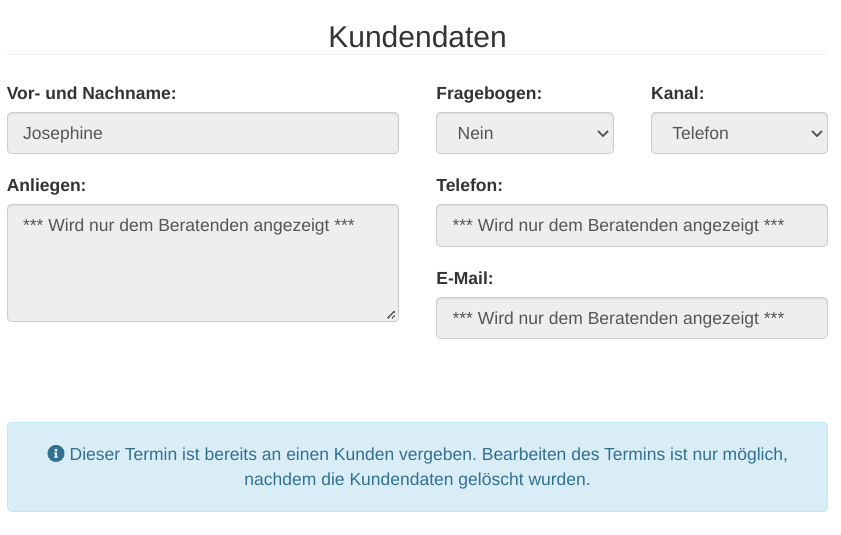
\includegraphics[width=0.9\textwidth]{screen_feedback_client_censorship.png}
\end{figure}


\begin{figure}[H]
    \caption{Neuer Button: Mit \textit{Speichern und Nächster} kann direkt der nächste Termin eingetragen werden.}
    \centering
    
\includegraphics[width=0.9\textwidth]{screen_feedback_save_next.png}
\end{figure}


\subsection{Reflektion der eingesetzen Methoden}

\paragraph{Human Centered Design und IIK}
% Einfache Umsetzung vs Nutzerfreundliche Lösung
% IIK sehr ertragreich, Prototypen wichtig für Feedback, Vorstellung

\paragraph{Implementierung und Usertests}
% Problem: Designpattern bei fertigem Softwareökosystem sehr eingeschränkt
% Fullcalendar Lib: Weniger Arbeit (billiger, robuster) dafür weniger Flexibilität
% Objektorientierter Ansatz sinnvoll für start serverlastige Anwendung?
% Evtl frühere Tests

\subsection{Zusammenfassender Abschluss}
% Eingehen auf Fragestellung der Einleitung
    % An welchen Stellen können die theoretischen Grundlagen des Human Centered Design den Entwicklungsprozess in der Praxis tatsächlich sinnvoll unterstützen? 
    % Gab es eventuell auch Methoden, die in der praktischen Umsetzung problematisch waren oder noch optimiert werden könnten?
    % Erfüllt die Software die gewünschten Anforderungen?
% Abrundendes Schlusswort

\subsection{Ausblick}
% Einführung neue Softwareversion (viel testen und abstimmen)
% Andere Module Überarbeiten
% Gruppentermine / Self Service einbuchen (Sicherheit)